\documentclass[12pt]{article}
\usepackage[]{graphicx}
\usepackage{newtxtext}
\pagestyle{empty}
\begin{document}
\vspace*{-2cm}
\noindent HW \#1 
\\ B455 Princples of Machine Learning 
\\ Professor Külekci
\\ January 20, 2024
\\\\Question 1:
\\\\\indent a. VC dimensions measure the learning capacity of the hypothesis by using 'shattering.'
For example, we have several points, N, which are either positive or negative, depending on the data.
when they need to determine a way to separate these points into their 'areas' of negative and positive only, without
having any errors. 
\\\\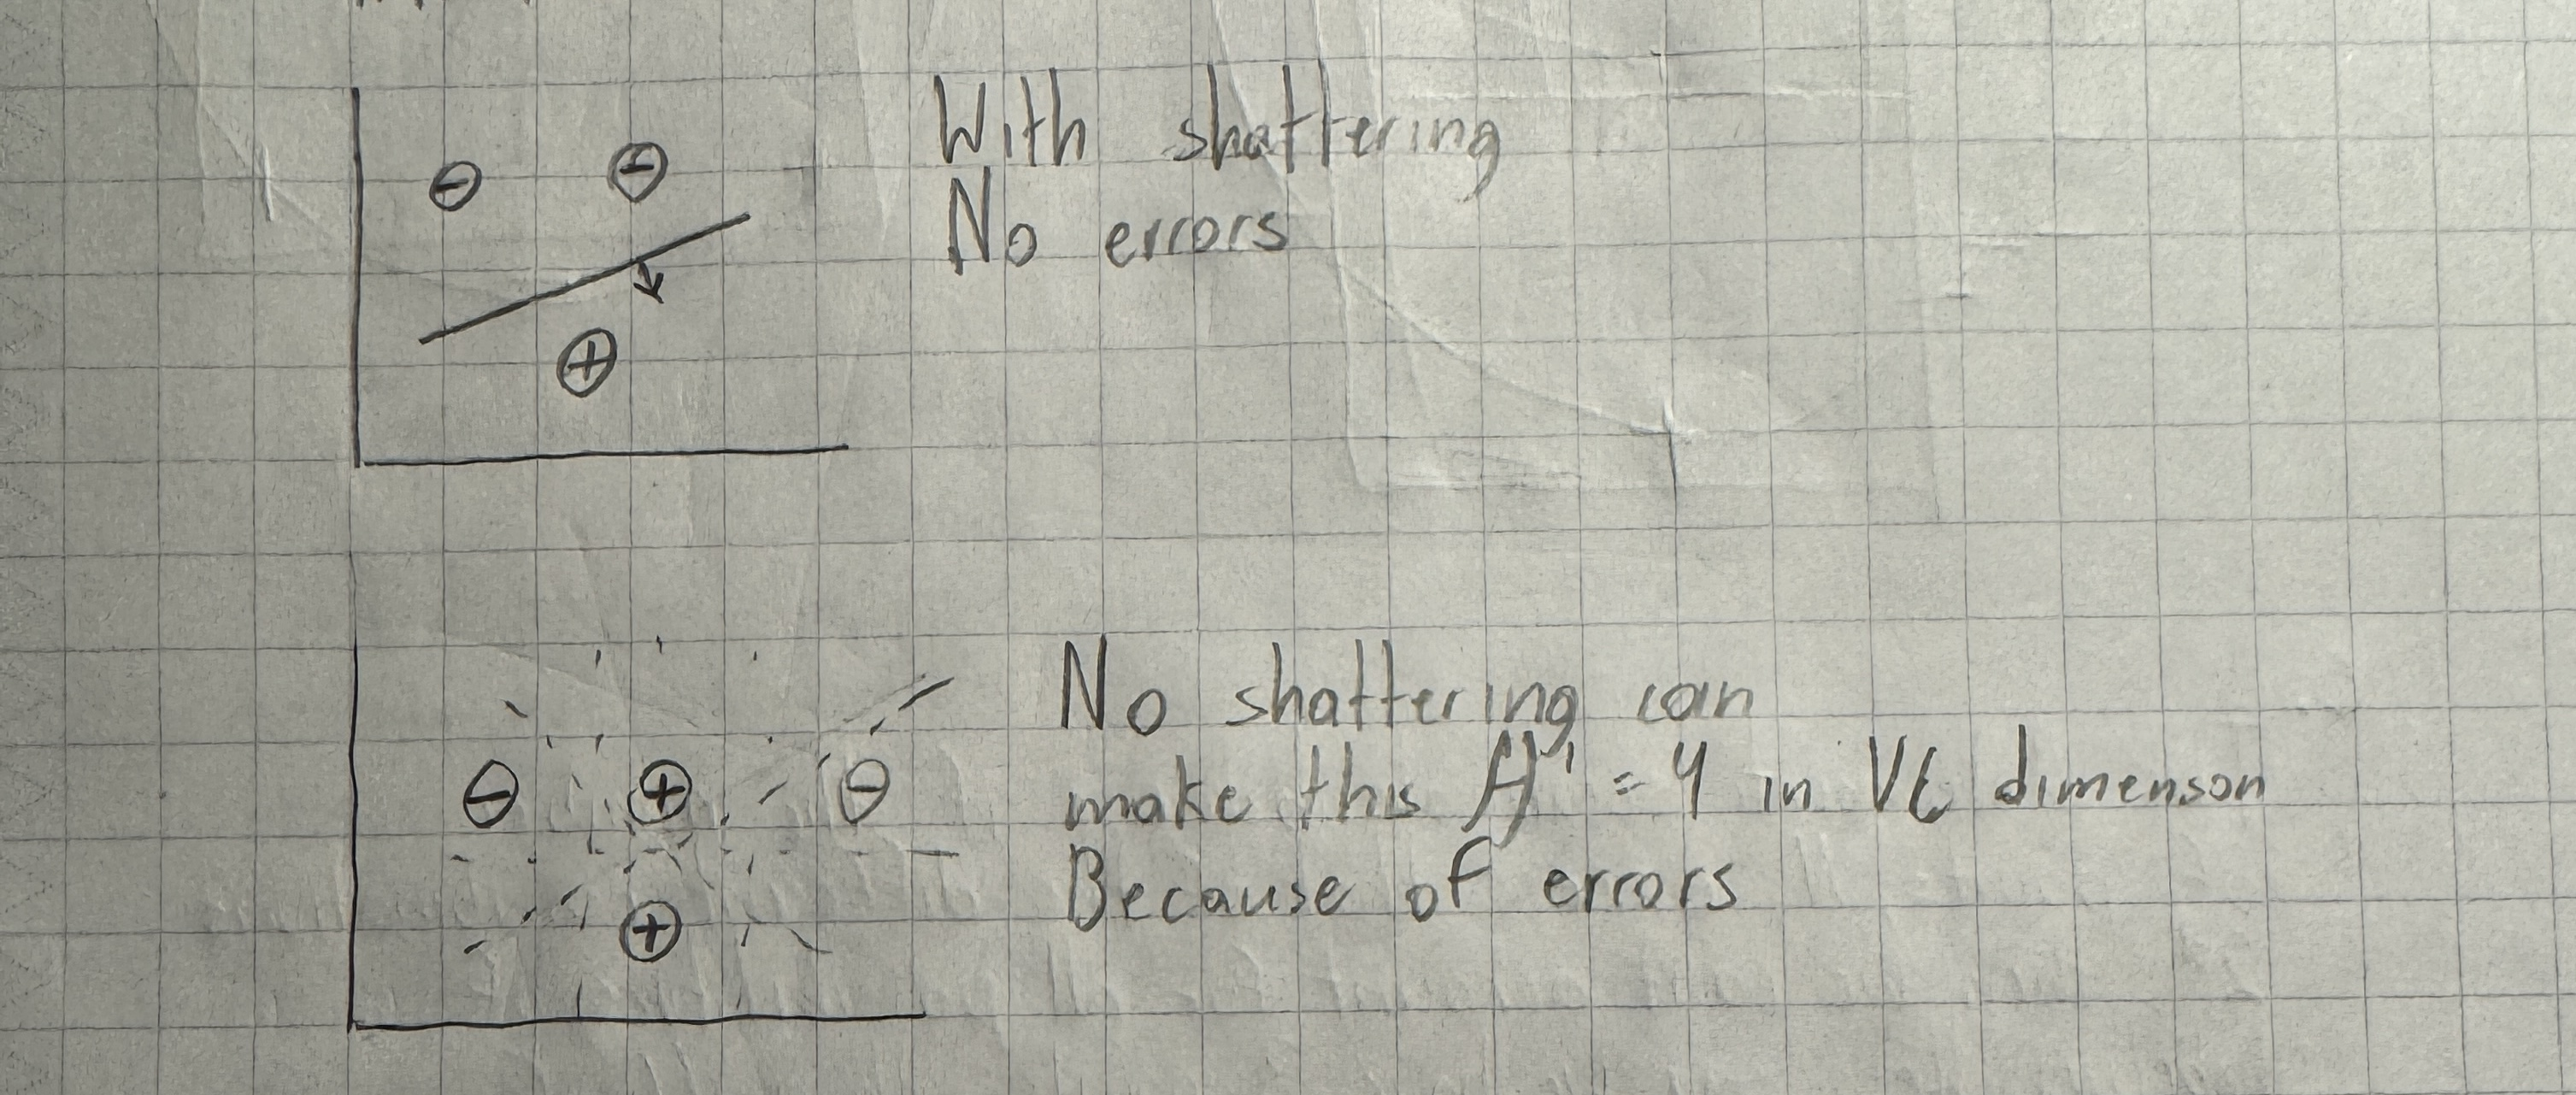
\includegraphics[scale=.54]{q1.jpg}
\\\\\indent b. Assuming the eight data points are in the position, like in the first photo,
the triangle would fit. Yet, a rectangle seems to be a better fit. The points can be in random positions, instead of 
one certain position, and would still fit, with less error, more examples can be seen in the second photo.\newline
\\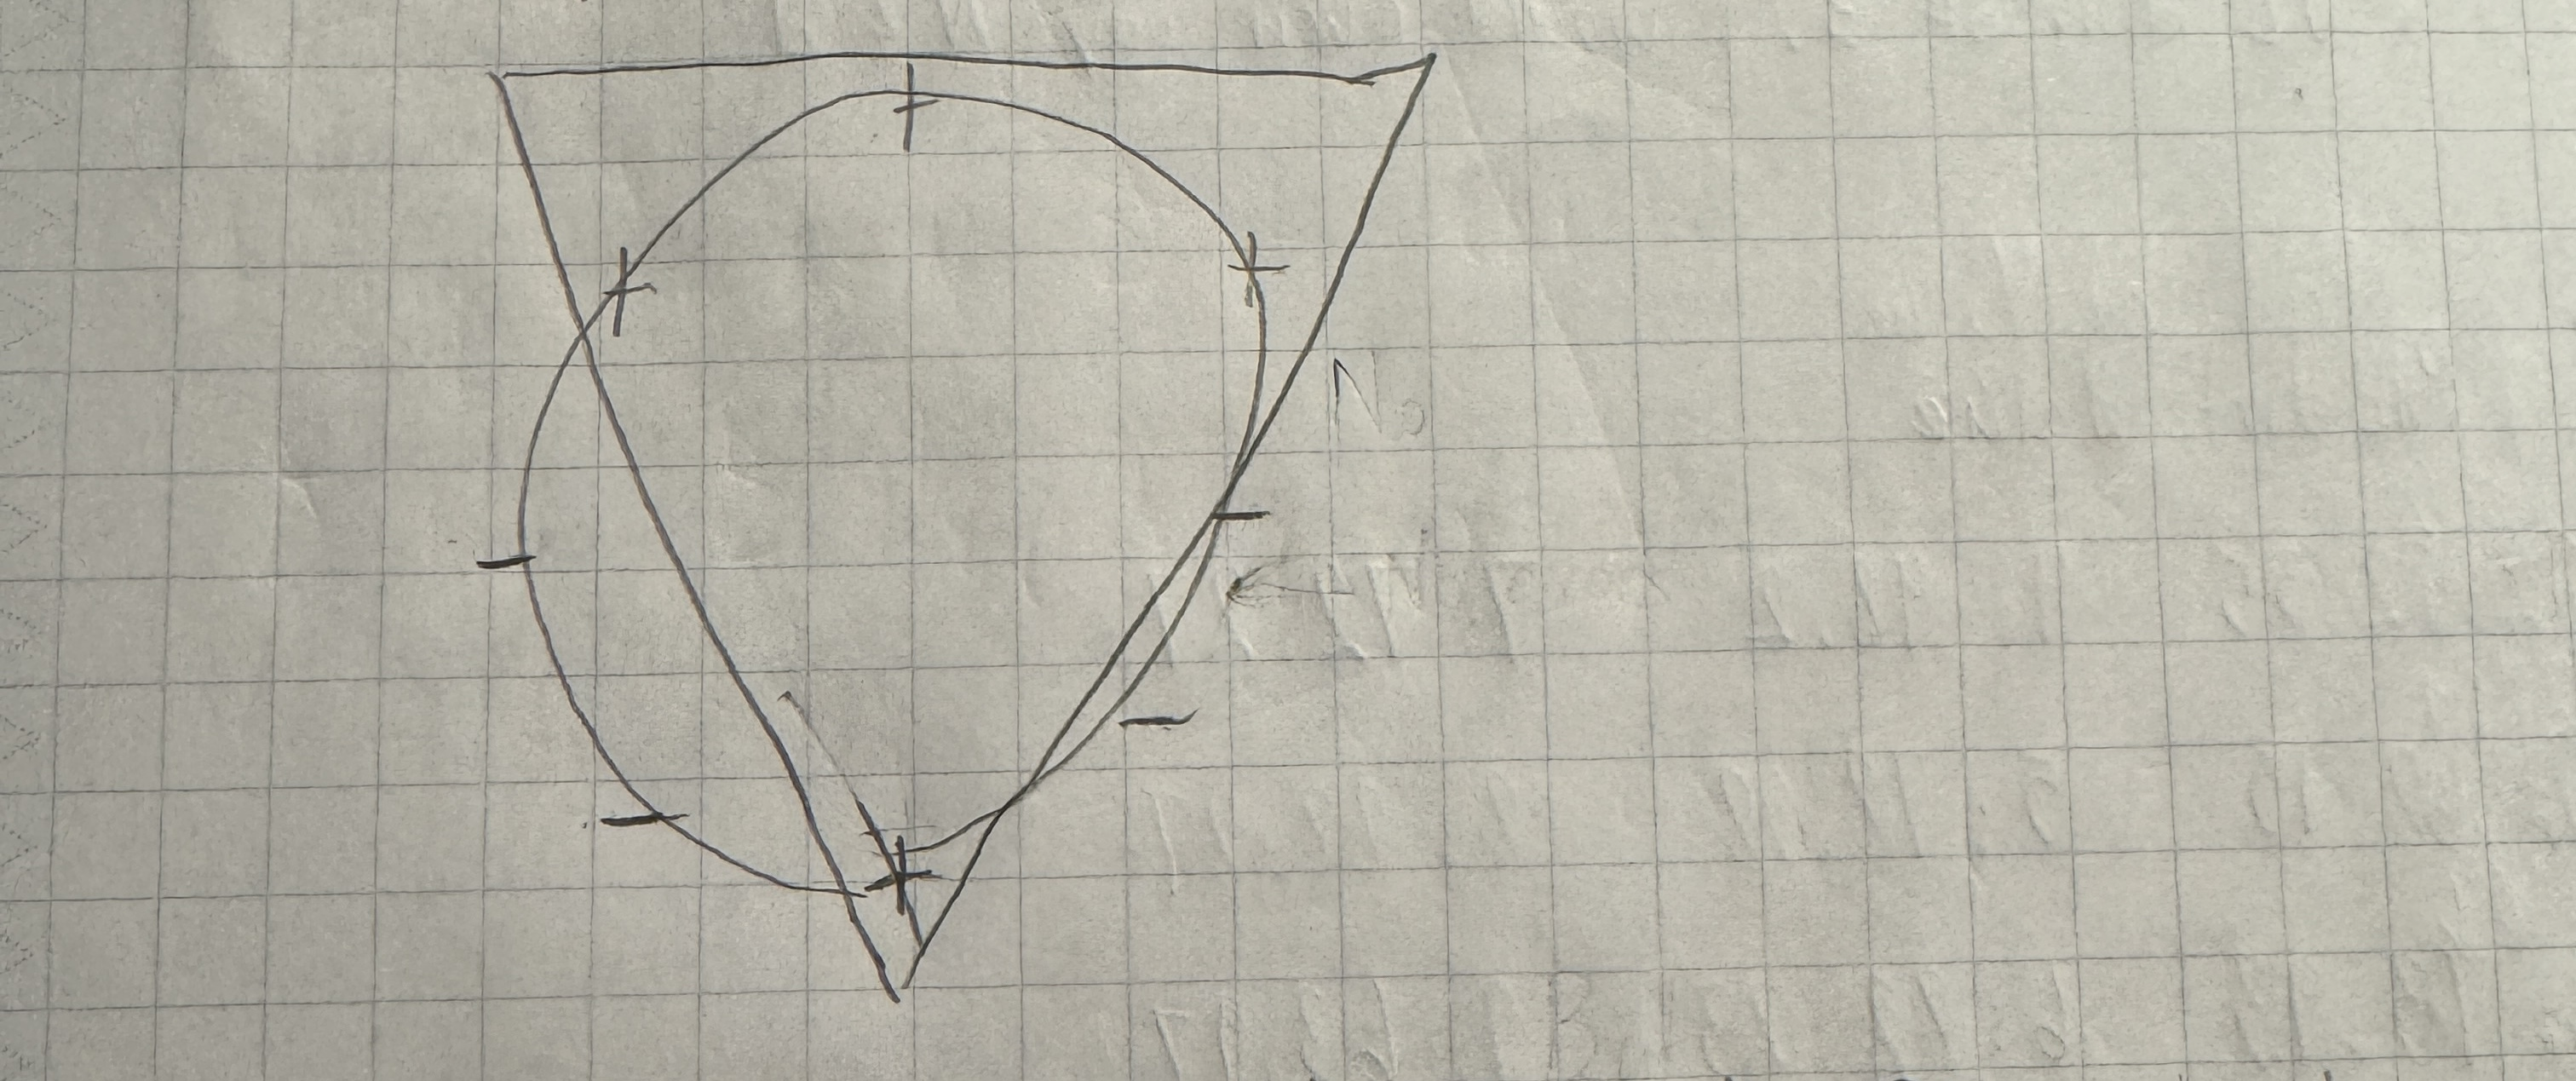
\includegraphics[scale=.54]{q1b.jpg}
\\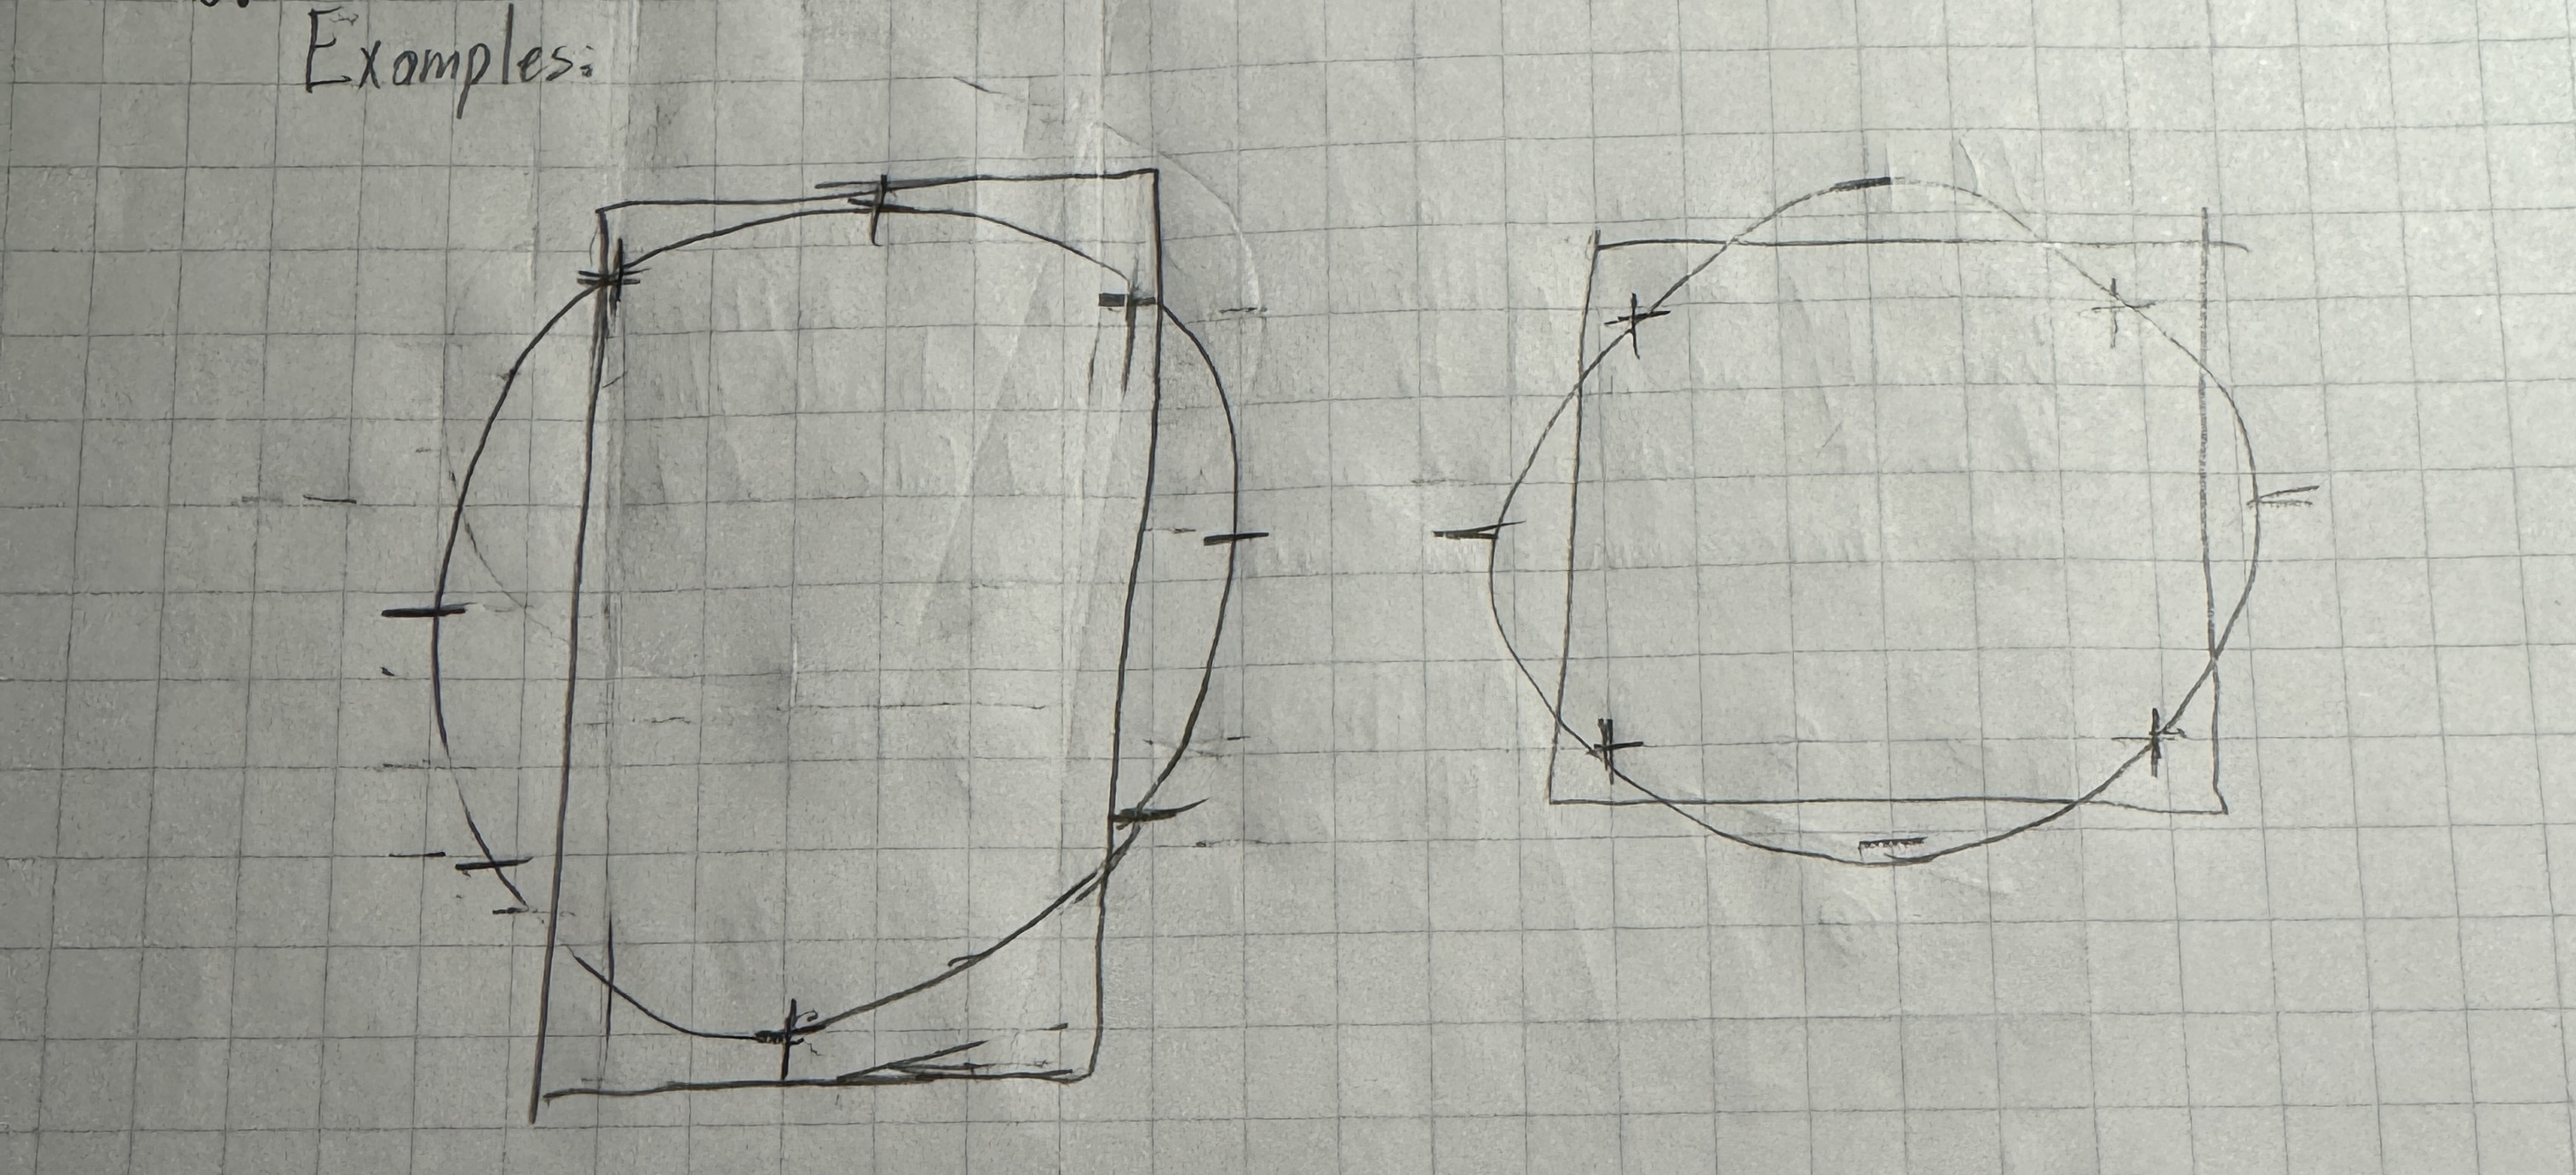
\includegraphics[scale=.54]{q1bII.jpg}
\\\\\indent c. The statement is accurate because if the number of points, $N$, exceeds that of the different 
combinations $2^d$, then we cannot account for all possibilities.
 Let's say we have three points with a VC of 3, so $3 \leq 2^3$. 
We can cover all the eight possibilities of those three points. 
If we did something like N=9 then we cannot cover all the possibilities with a VC of three, I would even say $N \leq d$.
\newpage
\vspace*{-1cm}
\noindent Question 2:
\begin{table}[h]
    \centering
    \begin{tabular}{|c|c|}
    \hline
    Exam & Predicted \\
    \hline
    1 & 52.35 \\
    2 & 68.95 \\
    3 & 73.93 \\
    4 & 48.2 \\
    5 & 78.08 \\
    6 & 82.23 \\
    7 & 72.27 \\
    8 & 88.87 \\
    9 & 63.97 \\
    \hline
    \end{tabular}
    \caption{Predicted Values}
\end{table}
\\\indent\textit{Note this was calulcated using the values from the table, given to us, results column: $predicted\_result = (0.83 * actual\_result)+15$}
\begin{table}[h]
    \centering
    \begin{tabular}{|c|c|c|}
    \hline
    Exam & Difference & Difference$^2$ \\
    \hline
    1 & 7.35 & 54.0225 \\
    2 & 3.96 & 15.6816 \\
    3 & 2.93 & 8.5849 \\
    4 & 8.2 & 67.24\\
    5 & 2.08 & 4.3264 \\
    6 & 1.23 & 1.5129 \\
    7 & 3.27 & 10.6929 \\
    8 & -0.13 & 0.0169 \\
    9 & 4.97 & 24.7009 \\
    \hline
    \end{tabular}
    \caption{Difference of Predicted and Actual}
\end{table}
\indent Once we have all the values of Difference$^2$, we take the sum and multipliy to find the error values. 
$Error\_Value=1/9($sum of Difference$^2) = 20.755$. Given this error amount, I would say it's a good amount of error, assuming that
this is 20.76\%. Because not all predictions will always result in 100\% accuracy. Even as humans, our predictions and performance, we have about the same amount of error more or less. 
Could it be improved? Yes, whether it's providing more cases, practice data, or adjusting/improving the algorithm, but I would say it's good for now.
\newpage
\vspace*{-1cm}
\noindent Question 3:
\\\\\indent a. We want to 'train' our model to learn what it should look for, what to calculate, or determine/evaluate. 
After we see the performance of the model, we adjust the model or select a different model to see if it performs better, which is the validation step. 
Finally, test to see the accuracy or scoring of our final model.
 Kind of like an exam, we learn definitions and practice the concepts in homework. 
Then take a practice exam to see what we need to improve, and finally the actual exam. 
\\\\\indent b. The model isn't learning in this case if it's just using training data. It's more like memorizing the data and then 'answers' to the data. 
Take for example a vocabulary test, all we are doing is memorizing the word over and over. 
It's not learning just memorizing the word's pronunciation and spelling, which is what the model is doing.
\end{document}